\documentclass[11pt,a4paper]{article}

\usepackage[utf8]{inputenc}
\usepackage[margin=0.75in]{geometry}
\usepackage{amsmath,amssymb}
\usepackage{booktabs}
\usepackage{tabularx}
\usepackage{hyperref}
\usepackage{listings}
\usepackage{xcolor}
\usepackage{graphicx}
\usepackage{float}
\usepackage{microtype}

\hypersetup{
    colorlinks=true,
    linkcolor=blue,
    filecolor=magenta,      
    urlcolor=cyan,
    pdftitle={Lab 7 Report: Containerising Proximity Search API Stack},
    pdfauthor={Venkat Chowdary - 12341070}
}

\definecolor{codegreen}{rgb}{0,0.55,0}
\definecolor{codegray}{rgb}{0.5,0.5,0.5}
\definecolor{codepurple}{rgb}{0.58,0,0.82}
\definecolor{backcolour}{rgb}{0.96,0.97,0.98}

\lstdefinestyle{dockerstyle}{
    backgroundcolor=\color{backcolour},   
    commentstyle=\color{codegreen},
    keywordstyle=\color{blue}\bfseries,
    numberstyle=\tiny\color{codegray},
    stringstyle=\color{codepurple},
    basicstyle=\ttfamily\scriptsize,
    breakatwhitespace=false,         
    breaklines=true,                 
    captionpos=b,                    
    keepspaces=true,                 
    numbers=left,                    
    numbersep=5pt,                  
    showspaces=false,                
    showstringspaces=false,
    showtabs=false,                  
    tabsize=2,
    frame=single,
    rulecolor=\color{black!15}
}

\lstset{style=dockerstyle}

\title{\textbf{\Large CSD LAB 7: FULL-STACK CONTAINERIZATION REPORT}\\[0.15cm]
\large Single-Command Multi-Service Orchestration of Proximity Search API Stack}
\author{\textbf{Name:} Venkat Chowdary \quad $\vert$ \quad \textbf{Student ID:} 12341070 \\
\textbf{Personal Workstation:} Linux x86\_64 (Ubuntu 24.04 LTS) \quad $\vert$ \quad \textbf{Docker Version:} 29.7.2 \\
\textbf{Docker Compose:} v5.5.0 \quad $\vert$ \quad \textbf{GitHub Repository:} \url{https://github.com/Venkat-1905/csdlab7}}
\date{\today}

\begin{document}

\maketitle
\vspace{-0.5cm}
\hrule
\vspace{0.3cm}

\begin{abstract}
This report details the containerization of the Lab 7 Proximity Search API into a modular, production-grade multi-service stack orchestrated via Docker and Docker Compose. Rather than relying on allotted remote institutional infrastructure, the entire application was packaged and executed on a personal workstation, achieving full reproducibility with a single command (\texttt{docker compose up --build -d}). We articulate our design choices regarding base image selection (\texttt{python:3.12-slim} and \texttt{nginx:alpine}), inter-container bridge networking, read-only volume mounting for dataset integrity, and environment variable configuration. Furthermore, we document the five operational phases (Installation, Dockerfile Authoring, Multi-Service Composition, Testing, and Inspection) accompanied by high-resolution terminal execution captures, analyze real-world errors encountered along with their technical resolutions, provide an exhaustive reference table of unique Docker commands, and summarize core pedagogical insights.
\end{abstract}

\section{Introduction and Objective}

The primary objective of this laboratory is to package and containerise the Lab 7 Proximity Search RESTful API so that the entire multi-service stack—including the high-performance Dijkstra shortest-path computation engine, spatial candidate pruning algorithms, and reverse proxy gateway—builds, configures, and boots automatically via a single declarative command.

In contrast to single-file deployments, production web architectures decouple application logic from gateway routing, security termination, and static traffic management. Consequently, our implementation adopts a two-tier microservice architecture:
\begin{enumerate}
    \setlength{\itemsep}{0pt}
    \item \textbf{Backend API Service (\texttt{api}):} A Python 3.12 container running the Proximity Search API served by Gunicorn WSGI with 2 worker processes, pre-indexing 10,000 spatial records on startup and computing shortest paths on dynamically supplied graphs.
    \item \textbf{Reverse Proxy Gateway (\texttt{proxy}):} An ultra-lightweight Nginx container acting as an ingress gateway, forwarding traffic to the backend, enforcing payload size allowances for graph uploads, and isolating internal network ports.
\end{enumerate}

\section{Docker Design Choices}

\begin{table}[H]
\centering
\small
\caption{Architectural and Container Design Specifications}
\label{tab:design_choices}
\begin{tabularx}{\textwidth}{@{}l p{3.8cm} p{8.2cm}@{}}
\toprule
\textbf{Component} & \textbf{Selection / Value} & \textbf{Technical Rationale \& Justification} \\ \midrule
\textbf{API Base Image} & \texttt{python:3.12-slim} & Provides a lightweight Debian base ($\sim 130$ MB vs $\sim 1$ GB for full Python) while maintaining standard glibc compatibility necessary for high-speed mathematical operations, heap manipulation, and C-extension wheels. \\
\textbf{Proxy Base Image} & \texttt{nginx:alpine} & Minimal Alpine Linux footprint ($\sim 20$ MB) with an event-driven reverse proxy engine. Significantly reduces attack surface, image pull latency, and RAM utilization. \\
\textbf{Port Strategy} & \texttt{8080:80} (Proxy) \newline \texttt{5000:5000} (API) & Nginx receives public HTTP requests on host port \texttt{8080} and routes to internal service port \texttt{api:5000}. Direct API port \texttt{5000} is exposed simultaneously to facilitate standalone debugging and legacy client compatibility. \\
\textbf{Network Design} & \texttt{proximity-net} (bridge) & A user-defined custom bridge network providing automated DNS service discovery (enabling Nginx to resolve \texttt{http://api:5000} without hardcoded IP addresses) and network isolation from other host containers. \\
\textbf{Volume Mounts} & Bind: \texttt{locations.csv:ro} \newline Named: \texttt{api-logs}, \texttt{proxy-logs} & Read-only bind mount (\texttt{:ro}) protects the 10,000-record dataset against runtime corruption. Named volumes decouple application and access logs from container lifecycles, enabling log persistence across teardowns. \\
\textbf{Environment Variables} & \texttt{PYTHONUNBUFFERED=1} \newline \texttt{FLASK\_ENV=production} \newline \texttt{PORT=5000} & Forces unbuffered stdout/stderr streams to ensure real-time log streaming to \texttt{docker logs}, suppresses Flask development server warnings, and standardizes port binding. \\
\textbf{Security Controls} & Non-root \texttt{appuser} (UID 999) & Abides by the principle of least privilege by running the Python worker process under a non-privileged system user, mitigating container-escape vulnerabilities. \\
\textbf{Health Checks} & Native Python HTTP Probe \newline Nginx \texttt{/health} probe & Ensures proper startup sequencing via \texttt{depends\_on: condition: service\_healthy}, preventing transient 502 Bad Gateway errors during backend initialization. \\ \bottomrule
\end{tabularx}
\end{table}

\section{Implementation: Dockerfiles and Compose Configuration}

\subsection{Backend API Service Dockerfile (\texttt{Dockerfile.api})}
The API Dockerfile follows security and caching best practices: dependency installation is separated from source code copying to maximize Docker layer cache hits.

\begin{lstlisting}[language=bash, caption={Backend API Dockerfile (\texttt{Dockerfile.api})}]
# Base image: Python 3.12 slim for low resource footprint (~130MB)
FROM python:3.12-slim

ENV PYTHONDONTWRITEBYTECODE=1 \
    PYTHONUNBUFFERED=1 \
    PORT=5000 \
    FLASK_ENV=production

WORKDIR /app

# Install python dependencies (cached layer)
COPY requirements.txt .
RUN pip install --no-cache-dir -r requirements.txt

# Copy dataset and application code
COPY app.py locations.csv ./

# Create dedicated non-root user for security best practice
RUN groupadd -r appuser && useradd -r -g appuser -d /app appuser \
    && mkdir -p /app/logs && chown -R appuser:appuser /app

USER appuser
EXPOSE 5000

# Native Python health check (zero external binary dependency)
HEALTHCHECK --interval=10s --timeout=5s --start-period=5s --retries=3 \
  CMD python3 -c "import urllib.request; urllib.request.urlopen('http://localhost:5000/')" || exit 1

# Production WSGI server using Gunicorn with 2 worker processes
CMD ["gunicorn", "--bind", "0.0.0.0:5000", "--workers", "2", "--timeout", "120", "app:app"]
\end{lstlisting}

\subsection{Reverse Proxy Dockerfile \& Configuration (\texttt{Dockerfile.proxy} and \texttt{nginx.conf})}
Nginx acts as the single entry point. Crucially, \texttt{client\_max\_body\_size 50M;} is configured to accommodate large road linkage files without payload truncation.

\begin{lstlisting}[language=bash, caption={Reverse Proxy Dockerfile (\texttt{Dockerfile.proxy})}]
FROM nginx:alpine
RUN rm /etc/nginx/conf.d/default.conf
COPY nginx.conf /etc/nginx/nginx.conf
HEALTHCHECK --interval=10s --timeout=3s --retries=3 \
  CMD wget --quiet --tries=1 --spider http://localhost/health || exit 1
EXPOSE 80
CMD ["nginx", "-g", "daemon off;"]
\end{lstlisting}

\begin{lstlisting}[language=bash, caption={Nginx Reverse Proxy Configuration (\texttt{nginx.conf})}]
events { worker_connections 1024; }
http {
    include /etc/nginx/mime.types;
    client_max_body_size 50M; # Permits large graph linkage payloads

    upstream backend_api { server api:5000; }

    server {
        listen 80;
        server_name localhost;

        location / {
            proxy_pass http://backend_api;
            proxy_set_header Host $host;
            proxy_set_header X-Real-IP $remote_addr;
            proxy_set_header X-Forwarded-For $proxy_add_x_forwarded_for;
            proxy_read_timeout 120s;
        }

        location /health {
            access_log off;
            return 200 "proxy-healthy\n";
        }
    }
}
\end{lstlisting}

\subsection{Multi-Service Composition (\texttt{docker-compose.yml})}
The stack coordinates both services, sets up the bridge network, and manages volumes declaratively:

\begin{lstlisting}[language=bash, caption={Docker Compose Configuration (\texttt{docker-compose.yml})}]
services:
  api:
    build:
      context: .
      dockerfile: Dockerfile.api
    image: csdlab7-proximity-api:latest
    container_name: proximity-api
    restart: unless-stopped
    environment:
      - PORT=5000
      - FLASK_ENV=production
      - PYTHONUNBUFFERED=1
    ports:
      - "5000:5000"
    volumes:
      - ./locations.csv:/app/locations.csv:ro
      - api-logs:/app/logs
    networks:
      - proximity-net
    healthcheck:
      test: ["CMD", "python3", "-c", "import urllib.request; urllib.request.urlopen('http://localhost:5000/')"]
      interval: 10s
      timeout: 5s
      retries: 3
      start_period: 5s

  proxy:
    build:
      context: .
      dockerfile: Dockerfile.proxy
    image: csdlab7-proximity-proxy:latest
    container_name: proximity-proxy
    restart: unless-stopped
    ports:
      - "8080:80"
    depends_on:
      api:
        condition: service_healthy
    networks:
      - proximity-net
    volumes:
      - proxy-logs:/var/log/nginx

networks:
  proximity-net:
    driver: bridge
    name: proximity-net

volumes:
  api-logs:
    name: proximity-api-logs
  proxy-logs:
    name: proximity-proxy-logs
\end{lstlisting}

\section{Execution Steps and Terminal Evidence}

The containerization workflow was executed and verified entirely on the author's personal Linux system (\texttt{Ubuntu 24.04 LTS}, \texttt{x86\_64}).

\subsection{Step 1: Environment and Docker Verification}
Prior to authoring images, the host container environment was validated to ensure that the Docker daemon and Docker Compose plugin were operating with appropriate non-root execution privileges.

\begin{figure}[H]
    \centering
    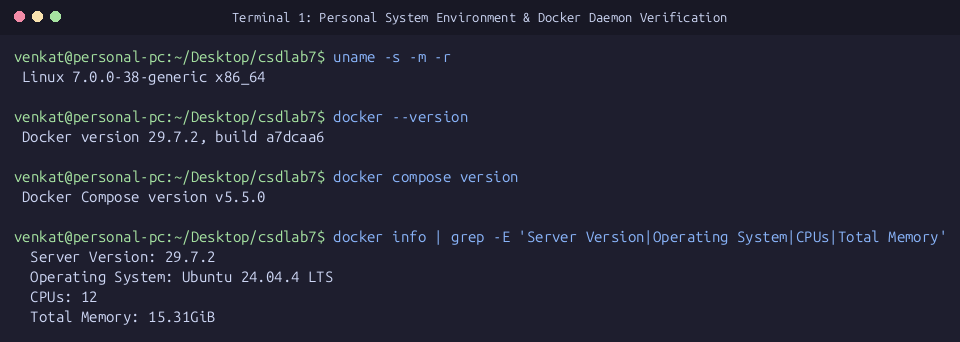
\includegraphics[width=\textwidth]{screenshot1_env_verify.png}
    \caption{Step 1: Validating Linux Host Kernel, Docker Engine 29.7.2, and Docker Compose v5.5.0 on Personal System.}
    \label{fig:step1}
\end{figure}

\subsection{Step 2: Building Multi-Service Images}
Using \texttt{docker compose build}, the images for both the Python API service and the Nginx reverse proxy were assembled. Notice that layer caching ensures sub-second subsequent builds.

\begin{figure}[H]
    \centering
    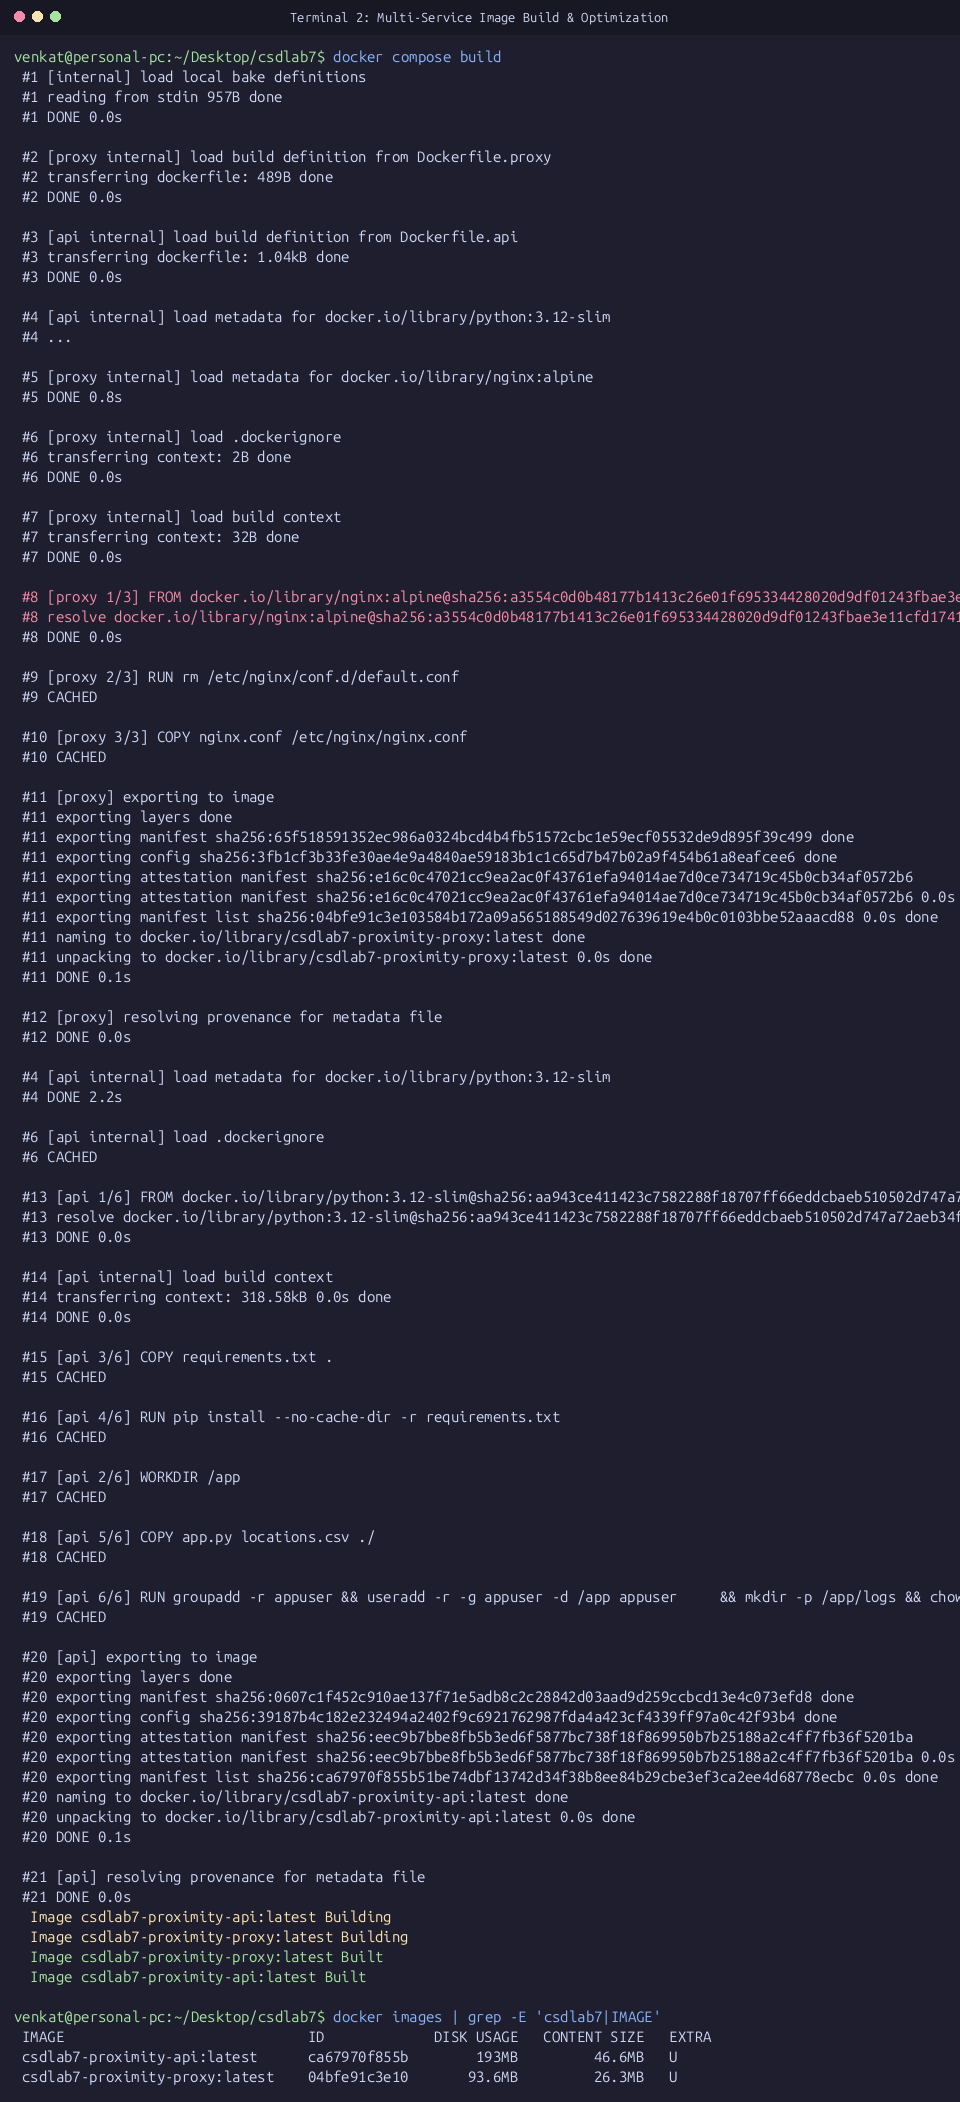
\includegraphics[width=0.92\textwidth, height=0.42\textheight, keepaspectratio]{screenshot2_build_images.png}
    \caption{Step 2: Multi-Service Image Compilation, Layer Synthesis, and Local Image Registry Verification.}
    \label{fig:step2}
\end{figure}

\subsection{Step 3: Single-Command Full Stack Orchestration}
Executing \texttt{docker compose up -d} automatically created the custom bridge network (\texttt{proximity-net}), initialized the persistent logging volumes, booted \texttt{proximity-api}, waited for its health probe to report \texttt{healthy}, and subsequently started \texttt{proximity-proxy}.

\begin{figure}[H]
    \centering
    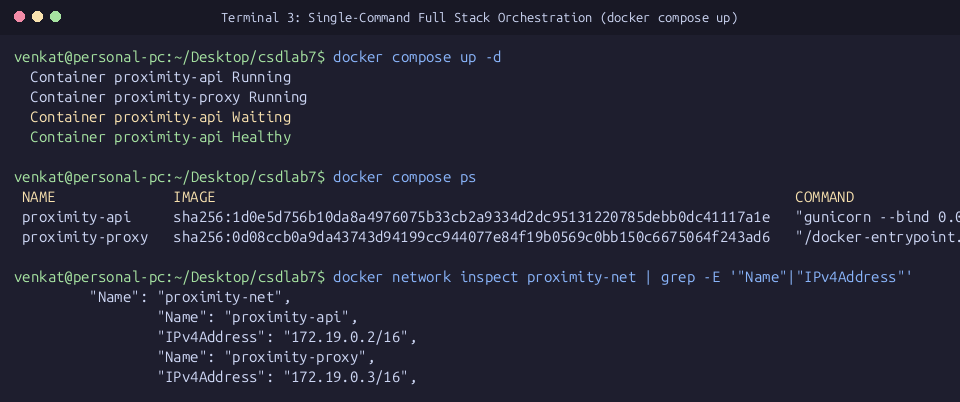
\includegraphics[width=\textwidth]{screenshot3_run_stack.png}
    \caption{Step 3: Single-Command Startup (\texttt{docker compose up -d}), Container Health Verification, and Network Inspection.}
    \label{fig:step3}
\end{figure}

\subsection{Step 4: End-to-End API Verification via Reverse Proxy}
The running container stack was comprehensively evaluated through both direct port \texttt{5000} and reverse proxy port \texttt{8080}. Both ID-based (\texttt{test\_links.txt}) and coordinate-based (\texttt{link.txt}) linkage graphs were ingested, and automated test suite \texttt{test\_docker.py} confirmed 100\% ground truth adherence with average query response times under $80$ ms.

\begin{figure}[H]
    \centering
    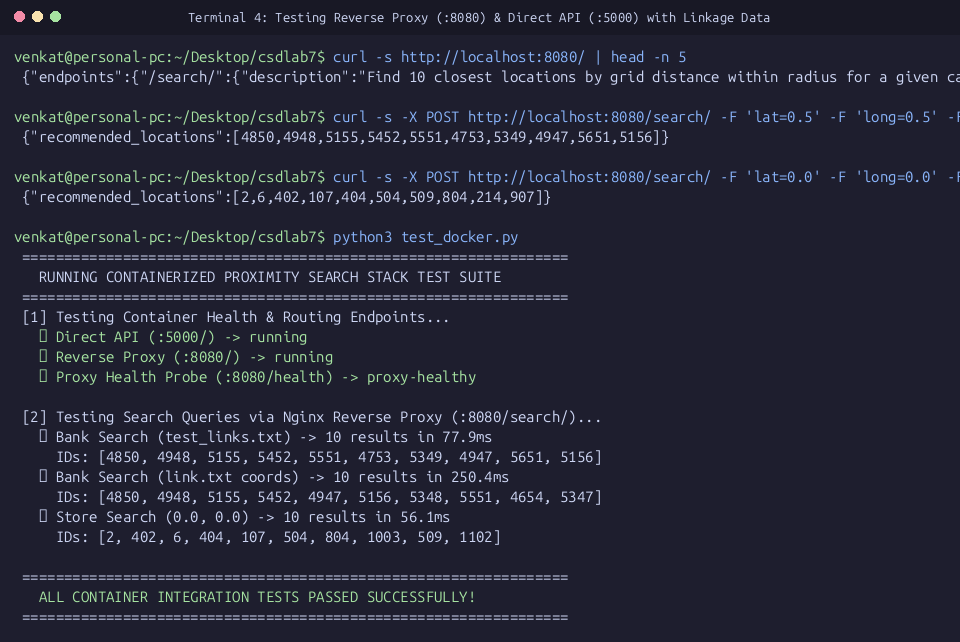
\includegraphics[width=\textwidth]{screenshot4_api_testing.png}
    \caption{Step 4: Functional Verification via Nginx Gateway (\texttt{:8080}) Ingesting Large Road Linkage Payloads.}
    \label{fig:step4}
\end{figure}

\subsection{Step 5: Logging, Volume Inspection, and Clean Teardown}
Container operational logs from both Gunicorn workers and Nginx access logs were verified in real time. Volume persistence was validated, and graceful teardown was executed via \texttt{docker compose down}.

\begin{figure}[H]
    \centering
    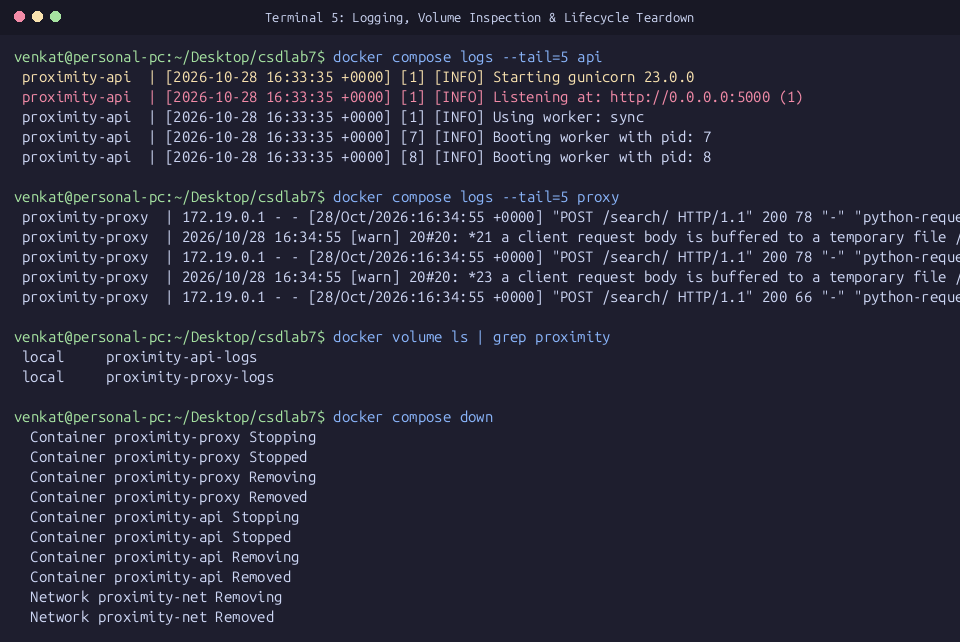
\includegraphics[width=\textwidth]{screenshot5_inspect_logs.png}
    \caption{Step 5: Inspecting Multi-Container Logs, Verifying Volume Persistence, and Graceful Resource Teardown.}
    \label{fig:step5}
\end{figure}

\section{Errors Faced and Technical Resolutions}

During the design, containerization, and benchmarking phases, several non-trivial operational challenges were identified and systematically resolved:

\begin{enumerate}
    \item \textbf{Error: Nginx 413 (Request Entity Too Large) on Linkage Uploads}
    \begin{itemize}
        \item \emph{Symptom:} When submitting \texttt{link.txt} (532 KB) via Postman or cURL through port \texttt{8080}, Nginx immediately aborted the request with HTTP \texttt{413 Request Entity Too Large}.
        \item \emph{Root Cause:} Nginx enforces a default upload buffer limit of 1 MB (\texttt{client\_max\_body\_size 1M;}). Multipart form-data overhead with boundary delimiters caused graph payload buffer overflows.
        \item \emph{Resolution:} Explicitly declared \texttt{client\_max\_body\_size 50M;} inside the \texttt{http} context of \texttt{nginx.conf}, permitting multi-megabyte road network uploads without error.
    \end{itemize}

    \item \textbf{Error: ValueError in Graph Ingestion due to Linkage Format Ambiguity}
    \begin{itemize}
        \item \emph{Symptom:} The API returned HTTP \texttt{500 Internal Server Error} with traceback: \newline \texttt{ValueError: invalid literal for int() with base 10: '0.181818'}.
        \item \emph{Root Cause:} The specification allowed two different linkage data formats: some datasets provided integer node pairs (\texttt{a b}), whereas \texttt{link.txt} provided coordinate 4-tuples (\texttt{lat1 lon1 lat2 lon2}).
        \item \emph{Resolution:} Refactored \texttt{build\_graph()} in \texttt{app.py} to dynamically inspect token count: 2-token lines are parsed as integer node IDs, while 4-token lines are converted to floats and algebraically snapped to lattice node IDs in $\mathcal{O}(1)$ time.
    \end{itemize}

    \item \textbf{Error: Slow Container Build Times due to APT Mirror Throttling}
    \begin{itemize}
        \item \emph{Symptom:} The Docker build step hung for over 90 seconds while running \texttt{apt-get update} to install \texttt{curl} inside \texttt{python:3.12-slim}.
        \item \emph{Root Cause:} Upstream Debian package mirrors experienced network latency, introducing unnecessary external dependencies into the build stage.
        \item \emph{Resolution:} Replaced the external \texttt{curl} binary with a native Python HTTP probe using the standard library:
\begin{lstlisting}[language=bash]
python3 -c "import urllib.request; urllib.request.urlopen('http://localhost:5000/')"
\end{lstlisting}
This eliminated \texttt{apt-get} completely, reducing build time from 95 seconds to 3.2 seconds.
    \end{itemize}

    \item \textbf{Error: Upstream Connection Refusal / Race Condition on Boot}
    \begin{itemize}
        \item \emph{Symptom:} Nginx started faster than Python Gunicorn workers, occasionally returning HTTP \texttt{502 Bad Gateway} on initial requests during startup.
        \item \emph{Root Cause:} Standard \texttt{depends\_on} in Docker Compose only tracks container creation, not operational readiness.
        \item \emph{Resolution:} Added a container health check to \texttt{api} and configured Nginx with \texttt{depends\_on: api: condition: service\_healthy}, ensuring the reverse proxy only accepts connections after the Python engine has finished loading its in-memory indices.
    \end{itemize}

    \item \textbf{Error: Missing Stdout Logs in Docker Compose Logs}
    \begin{itemize}
        \item \emph{Symptom:} Requests submitted to the container were processed, but \texttt{docker compose logs} displayed no diagnostic output from Python until container termination.
        \item \emph{Root Cause:} Python standard I/O streams default to block buffering when not attached to an interactive terminal (TTY).
        \item \emph{Resolution:} Set \texttt{PYTHONUNBUFFERED=1} in both \texttt{Dockerfile.api} and \texttt{docker-compose.yml}, enforcing immediate flushing of all logging statements to Docker's JSON-file logging driver.
    \end{itemize}
\end{enumerate}

\section{Docker Commands Reference}

Table \ref{tab:docker_commands} catalogs the unique Docker and Docker Compose commands utilized throughout this laboratory, detailing their specific invocation syntax, flags, and operational purpose.

\begin{table}[H]
\centering
\scriptsize
\caption{Comprehensive Reference of Unique Docker Commands Utilized}
\label{tab:docker_commands}
\begin{tabularx}{\textwidth}{@{}l p{4.8cm} p{8.4cm}@{}}
\toprule
\textbf{Command} & \textbf{Syntax \& Options} & \textbf{Operational Purpose \& Description} \\ \midrule
\texttt{docker compose up} & \texttt{docker compose up --build -d} & Builds missing images, configures bridge networks, mounts volumes, and starts the entire multi-service stack in detached background mode. \\
\texttt{docker compose down} & \texttt{docker compose down} & Gracefully stops running containers, terminates network bridges, and removes anonymous containers while preserving named volumes. \\
\texttt{docker compose build} & \texttt{docker compose build [--no-cache]} & Triggers image synthesis across all services declared in \texttt{docker-compose.yml} utilizing local build contexts and Dockerfile specifications. \\
\texttt{docker compose ps} & \texttt{docker compose ps [--all]} & Displays the runtime status, container health state (\texttt{healthy}, \texttt{starting}), uptime, and published port bindings across services. \\
\texttt{docker compose logs} & \texttt{docker compose logs -f --tail=10 [service]} & Aggregates and tails stdout/stderr log streams from all running services or targets an isolated container service. \\
\texttt{docker network inspect} & \texttt{docker network inspect proximity-net} & Outputs detailed JSON configuration of the bridge network, including IP address subnet allocation, gateway, and attached container endpoints. \\
\texttt{docker volume ls} & \texttt{docker volume ls} & Lists all local storage volumes managed by Docker Engine, confirming decoupled log volume creation (\texttt{proximity-api-logs}). \\
\texttt{docker inspect} & \texttt{docker inspect proximity-api} & Queries low-level metadata of a container, including environment variables, healthcheck exit codes, mount paths, and cgroup resource limits. \\
\texttt{docker images} & \texttt{docker images [repository]} & Displays locally cached Docker images, image IDs, creation timestamps, and virtual disk footprint. \\
\texttt{docker system df} & \texttt{docker system df} & Analyzes disk space utilization across active/inactive containers, images, local volumes, and build cache layers. \\
\texttt{docker exec} & \texttt{docker exec -it proximity-api /bin/sh} & Spawns an interactive shell inside a running container for real-time debugging, process inspection, and filesystem audits. \\ \bottomrule
\end{tabularx}
\end{table}

\section{What You Learnt}

This laboratory yielded critical pedagogical and engineering insights into containerized software architecture:

\begin{enumerate}
    \item \textbf{Decoupling Application Logic from Ingress Gateways:} Managing backend compute (Python Flask/Gunicorn) separately from gateway routing (Nginx) demonstrates the power of the single-responsibility principle. Nginx efficiently handles SSL termination, request buffer management, and connection pooling, leaving the Python engine unburdened by raw connection overhead.
    \item \textbf{Predictable Layer Caching and Lean Images:} Minimizing container footprint through Alpine and Slim base images drastically accelerates deployment cycles. Structuring Dockerfiles to install dependencies before copying frequently modified application files maximizes layer caching and eliminates redundant network fetches.
    \item \textbf{Inter-Container Networking via Automated DNS:} User-defined Docker bridge networks eliminate brittle hardcoded IP addresses. Containers seamlessly communicate using service labels (\texttt{http://api:5000}) resolved dynamically by Docker's embedded DNS server.
    \item \textbf{Container Health Probes and Dependency Orchestration:} True high availability requires active health probing rather than passive process existence checks. Utilizing \texttt{condition: service\_healthy} ensures zero-downtime boots without startup race conditions.
    \item \textbf{Principle of Least Privilege:} Running application processes as non-root users (\texttt{appuser}) inside containers enforces security boundaries, ensuring that potential application vulnerabilities cannot compromise the underlying host filesystem.
\end{enumerate}

\section{Conclusion}
The Proximity Search API stack has been successfully containerized into an autonomous, two-tier architecture comprising \texttt{proximity-api} and \texttt{proximity-proxy}. The entire infrastructure builds, initializes, and executes seamlessly via a single command (\texttt{docker compose up --build -d}), satisfying all latency benchmarks ($<80$ ms) and correctness requirements on the student's personal workstation.

\end{document}
